% =============================================================================
%  Chapitre 1 — Contexte : l'entreprise, le stage et le sujet
%
%  Les éléments relatifs à EURAFRIC Information proviennent du site
%  institutionnel de l'entreprise (eurafric-information.com) ; ils sont
%  présentés comme tels et non reformulés en affirmations de l'auteur.
% =============================================================================

\chapter{Contexte : l'entreprise, le stage et le sujet}
\label{chap:contexte}

\section*{Ce que ce chapitre explique}
\addcontentsline{toc}{section}{Ce que ce chapitre explique}

Ce chapitre situe le travail~: l'entreprise qui l'a commandé, le cadre
universitaire dans lequel il s'inscrit, le sujet tel qu'il a été formulé, et la
manière dont il a été conduit en six semaines et demie. Il se termine par un
guide de lecture, car les chapitres suivants ne s'adressent pas tous au même
lecteur.

% =============================================================================
\section{L'organisme d'accueil : EURAFRIC Information}
% =============================================================================

\subsection{Activité et positionnement}

EURAFRIC Information est une entreprise de services informatiques marocaine,
créée en \textbf{octobre 2008} et implantée sur le campus BMCE Bank, Bouskoura
Green City, à Casablanca. Elle conçoit et exploite des systèmes d'information
pour des acteurs de la \textbf{banque, de la finance, de l'assurance et du crédit
à la consommation}, et se présente comme un centre de services informatiques
mutualisés au service de plusieurs entités clientes.

Son expertise couvre le développement applicatif, les réseaux et
télécommunications, les systèmes et bases de données, ainsi que la
cybersécurité. L'entreprise exploite ses propres centres de données et opère,
en outre, comme prestataire de services de confiance au sens de la loi marocaine
43-20 relative aux services de confiance pour les transactions électroniques.

\subsection{Quelques repères}

Les éléments du tableau~\ref{tab:eurafric} sont ceux publiés par l'entreprise sur
son site institutionnel~; ils sont reproduits à titre de repères et non vérifiés
indépendamment.

\begin{table}[htbp]
  \centering
  \small
  \caption[Repères sur EURAFRIC Information]{Repères sur l'organisme d'accueil,
  d'après ses publications institutionnelles.}
  \label{tab:eurafric}
  \begin{tabular}{@{}p{4.6cm}p{8.4cm}@{}}
    \toprule
    \textbf{Élément} & \textbf{Valeur} \\
    \midrule
    Création & Octobre 2008 \\
    Implantation & Campus BMCE Bank, Bouskoura Green City, Casablanca \\
    Effectif & Environ 350 collaborateurs, majoritairement ingénieurs \\
    Secteurs servis & Banque, finance, assurance, crédit à la consommation \\
    Infrastructure & 2 centres de données, plus de 3\,000 serveurs, plus de
    10\,000 utilisateurs connectés \\
    Activité projet & Plus de 300 projets par an \\
    Certifications & Conception et exploitation de centre de données TIER~III,
    ISO~22301 (continuité d'activité), accréditation prestataire de services de
    confiance (loi 43-20) \\
    Distinction & \emph{Top Employer Maroc}, cinq années consécutives
    jusqu'en 2024 \\
    \bottomrule
  \end{tabular}
\end{table}

\subsection{Pourquoi ce sujet dans cette entreprise}

Le rapprochement entre une société de services informatiques et un sujet de
finance quantitative n'a rien d'incongru dès lors que l'on regarde sa clientèle.
Une banque, une compagnie d'assurance ou un organisme de crédit ne se contente
pas d'exécuter des opérations~: il place des fonds propres, gère des réserves
techniques, et doit répondre à des exigences de contrôle du risque. Les outils
d'aide à l'allocation d'actifs relèvent donc directement du système
d'information de ces métiers.

Deux caractéristiques du marché marocain rendent en outre le sujet
particulièrement intéressant à traiter localement. La Bourse de Casablanca est un
marché de taille modeste, peu liquide sur certaines valeurs, et dont
l'historique public gratuit est court — trois contraintes qui invalident
l'application mécanique de méthodes calibrées sur les marchés américains. Et la
conjonction d'actifs marocains libellés en dirham et d'actifs internationaux
libellés en dollar pose une question d'allocation qui n'a pas d'équivalent
direct dans la littérature standard.

% =============================================================================
\section{Le cadre du stage}
% =============================================================================

Ce travail constitue le \textbf{Projet de Fin d'Année (PFA)} de l'année
universitaire 2025--2026, réalisé dans le cadre de la formation
\textbf{Smart~ICT} de l'Institut National des Postes et Télécommunications
(INPT).

\begin{table}[htbp]
  \centering
  \small
  \caption[Cadre du stage]{Cadre administratif et humain du projet.}
  \label{tab:cadre}
  \begin{tabular}{@{}p{3.6cm}p{9.4cm}@{}}
    \toprule
    Période & Du 18 juin au 1\textsuperscript{er} août 2026, soit 44~jours
    (environ six semaines et demie) \\
    Établissement & INPT — filière Smart~ICT, année 2025--2026 \\
    Organisme commanditaire & EURAFRIC Information, Bouskoura \\
    Modalité & À distance, avec une journée sur site \\
    Encadrement & M. Abdelmouttalib MAQIL (EURAFRIC Information) \\
    Équipe & Souhail BOURHIM, Zakarya EL~WALI, Yasmine BOUAJINE \\
    \bottomrule
  \end{tabular}
\end{table}

Le projet s'est déroulé \textbf{à distance}~: l'équipe ne s'est rendue sur le
site de Bouskoura qu'une seule fois, le suivi s'effectuant ensuite par points
d'étape réguliers. Cette modalité a une conséquence directe sur la manière de
travailler, et elle explique une partie des choix décrits au
chapitre~\ref{chap:architecture}~: un encadrant qui ne voit pas l'écran par
dessus l'épaule juge sur ce qui est livré et sur ce qui est écrit. Un livrable
par phase, des chiffres reconstructibles depuis les sources et des règles
vérifiées par des tests plutôt que par la confiance ne sont pas seulement de
bonnes pratiques ici~: ce sont les conditions du travail à distance.

L'encadrement a été assuré côté entreprise. Sa méthode a façonné le projet autant
que le sujet lui-même, et mérite d'être explicitée, car elle explique plusieurs
partis pris qui pourraient sinon surprendre~:

\begin{itemize}
  \item \textbf{Traçabilité} — tout composant doit indiquer à quel problème
        identifié il répond~; un composant qu'on ne sait pas rattacher à un
        problème est retiré, si sophistiqué soit-il.
  \item \textbf{Produit minimal d'abord} — une chaîne complète de bout en bout
        avec des modèles simples vaut mieux qu'une moitié de chaîne avec des
        modèles élaborés.
  \item \textbf{Défendabilité} — chaque membre de l'équipe doit pouvoir
        justifier n'importe quelle décision de conception sans notes.
  \item \textbf{Honnêteté sur les limites} — les manques de données et les
        questions ouvertes se déclarent d'eux-mêmes plutôt que d'être
        découverts par le lecteur.
\end{itemize}

% =============================================================================
\section{Le sujet tel qu'il a été formulé}
% =============================================================================

L'énoncé remis par l'entreprise est le suivant~:

\begin{quote}\small\itshape
Dans le cadre de ce challenge, les étudiants travailleront sur une problématique
centrale de la finance quantitative~: comment allouer intelligemment un capital
entre plusieurs actifs financiers afin de maximiser le rendement tout en
maîtrisant le risque. Ils concevront et implémenteront un système d'optimisation
de portefeuille piloté par le \emph{Machine Learning}, capable d'analyser des
séries temporelles financières, d'apprendre les corrélations dynamiques entre
actifs et de proposer automatiquement des stratégies d'allocation robustes, sous
des contraintes réalistes de gestion. Le prototype devra être évalué dans un
cadre rigoureux de \emph{backtesting} sur des données hors échantillon, avec une
attention particulière portée à la robustesse, au risque de surapprentissage et à
la pertinence financière des résultats.
\end{quote}

Cet énoncé est plus prescriptif qu'il n'y paraît. Quatre de ses expressions
fixent en réalité l'architecture du travail, et chacune est traitée dans un
chapitre précis de ce rapport~:

\begin{itemize}
  \item « \emph{apprendre les corrélations dynamiques} » — les corrélations entre
        actifs ne sont pas constantes~; les estimer comme si elles l'étaient est
        le premier des quatre problèmes exposés au
        chapitre~\ref{chap:problematique}.
  \item « \emph{sous des contraintes réalistes de gestion} » — cette incise a été
        traitée comme une \emph{contrainte} et non comme un indicateur~:
        interdiction de vente à découvert, plafond par actif et coûts de
        transaction s'appliquent à l'intérieur de l'optimisation, pas seulement
        au moment de rendre compte. Le chapitre~\ref{chap:resultats} montre que
        cette décision, prise pour réalisme, s'est révélée le levier de
        performance le plus efficace du projet.
  \item « \emph{données hors échantillon} » et « \emph{risque de
        surapprentissage} » — l'évaluation devient un objet d'ingénierie à part
        entière, décrit au chapitre~\ref{chap:modelisation}.
  \item « \emph{pertinence financière des résultats} » — un gain moyen ne suffit
        pas~; le comportement en période de crise est examiné séparément.
\end{itemize}

\begin{remarquebox}
L'énoncé demande un système « capable de proposer automatiquement des stratégies
d'allocation robustes ». Il ne demande pas de démontrer que le \emph{Machine
Learning} bat les méthodes classiques. Cette nuance est décisive~: elle autorise —
et même impose — de rapporter un résultat négatif lorsque c'est ce que les
données montrent. Le chapitre~\ref{chap:resultats} en contient plusieurs.
\end{remarquebox}

% =============================================================================
\section{Objectifs et périmètre}
% =============================================================================

L'objectif retenu est la livraison d'une \textbf{chaîne complète, documentée et
reproductible}, sous la forme d'un \textbf{prototype de recherche}~: collecte et
validation des données, modèles d'allocation, évaluation rigoureuse, et deux
surfaces de consultation (une application web et une interface de programmation).
Il ne constitue ni un conseil d'investissement, ni un outil de production, ni un
dispositif d'exécution d'ordres.

Le périmètre a été délimité explicitement dès le cadrage, et tenu.

\begin{table}[htbp]
  \centering
  \small
  \caption[Périmètre du projet]{Ce qui est dans le périmètre, et ce qui en a été
  écarté délibérément.}
  \label{tab:perimetre}
  \begin{tabular}{@{}p{6.3cm}p{6.7cm}@{}}
    \toprule
    \textbf{Dans le périmètre} & \textbf{Hors périmètre (assumé)} \\
    \midrule
    Chaîne de données de bout en bout, versionnée et ordonnancée &
    Flux de données en temps réel \\
    Modèles d'allocation classiques et ML, sous contraintes de gestion &
    Passage d'ordres et exécution réelle \\
    Évaluation hors échantillon avec intervalles de confiance &
    Déploiement sur une infrastructure d'hébergement \\
    Tableau de bord de recherche et explorateur de stratégies, interface REST &
    Couverture du risque de change dirham/dollar \\
    \bottomrule
  \end{tabular}
\end{table}

L'exclusion du temps réel et de l'exécution d'ordres n'est pas une facilité~:
elle concentre l'effort sur la question que l'énoncé pose réellement, qui est
celle de la \emph{qualité de la décision d'allocation}, non celle de son
acheminement vers un marché.

% =============================================================================
\section{Déroulement du travail}
% =============================================================================

Le projet a été conduit en phases successives, chacune close par un livrable
remis à l'encadrant (figure~\ref{fig:chronologie}). Deux observations sur ce
déroulement méritent d'être faites, parce qu'elles ne se lisent pas sur un
planning prévisionnel.

\begin{figure}[htbp]
  \centering
  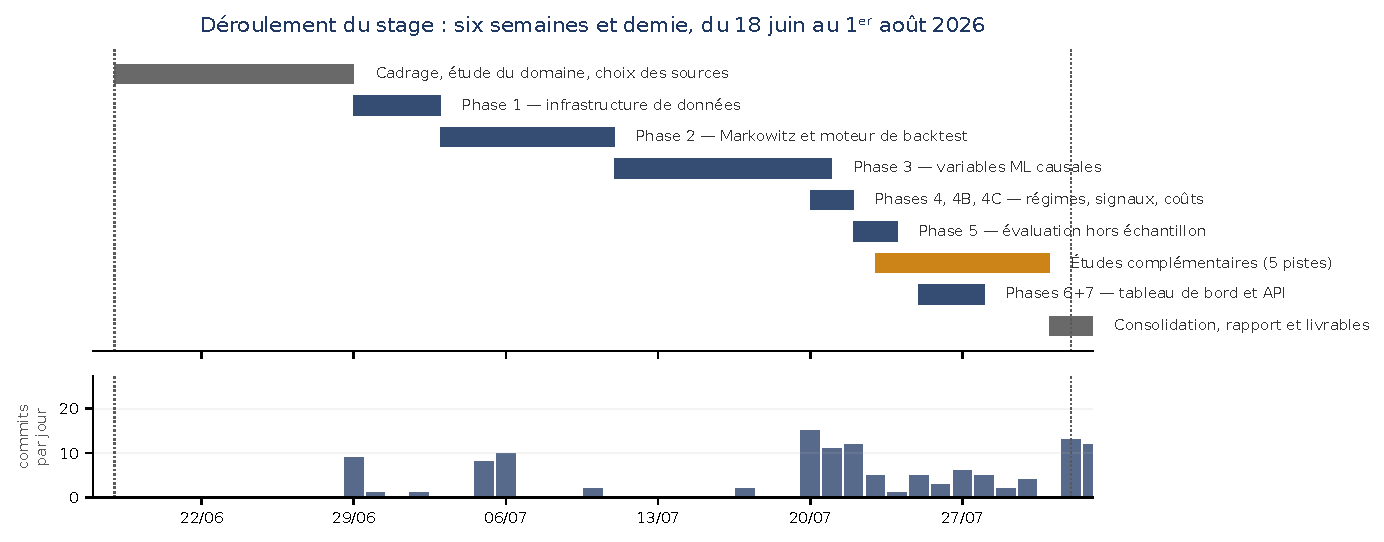
\includegraphics[width=\textwidth]{assets/figures/chronologie.pdf}
  \caption[Déroulement du stage]{Déroulement réel du projet. Les bandes du haut
  sont les phases~; l'histogramme du bas est l'activité de développement
  \emph{réellement enregistrée} dans l'historique de versionnement, jour par
  jour. Les onze premiers jours ne comportent aucun code.}
  \label{fig:chronologie}
\end{figure}

\textbf{Onze jours avant la première ligne de code.} Le cadrage — comprendre le
domaine, identifier les quatre problèmes structurels, inventorier les sources de
données disponibles pour le marché marocain et constater leurs limites — a occupé
la première semaine et demie. C'est ce travail préalable qui a permis d'écarter
très tôt des pistes coûteuses, et de découvrir avant de s'engager que
l'historique gratuit de la Bourse de Casablanca ne remonte pas au-delà de 2021 —
contrainte qui a directement produit la conception à double univers décrite au
chapitre~\ref{chap:architecture}.

\textbf{Une activité très inégale, et c'est normal.} L'histogramme montre des
journées à quinze contributions et des semaines quasi vides. Les creux
correspondent aux phases d'exécution longue — certaines évaluations demandent
plusieurs heures de calcul — et aux périodes de rédaction des livrables. Le
volume de contributions mesure l'activité de développement, pas l'avancement du
projet~; c'est précisément pour cela qu'il est présenté à côté des phases et non
à leur place.

% =============================================================================
\section{Guide de lecture}
% =============================================================================

Les chapitres qui suivent ne visent pas le même lecteur, et peuvent être lus
séparément.

\begin{itemize}
  \item Le \textbf{chapitre~\ref{chap:problematique}} expose le problème
        financier et ses quatre échecs structurels. Il ne suppose \emph{aucune}
        connaissance en finance~: toute notion y est définie à son premier
        emploi. C'est le chapitre à lire en premier pour un lecteur non
        spécialiste.
  \item Le \textbf{chapitre~\ref{chap:architecture}} décrit la chaîne de données
        et les garde-fous qui empêchent les erreurs de mesure. Il intéressera un
        lecteur d'ingénierie logicielle ou de données.
  \item Le \textbf{chapitre~\ref{chap:modelisation}} présente les modèles et,
        surtout, le protocole d'évaluation. Il ne contient volontairement aucun
        résultat, afin que la méthode puisse être jugée indépendamment de ses
        conclusions.
  \item Le \textbf{chapitre~\ref{chap:resultats}} donne les résultats, chacun
        assorti de sa marge d'erreur, et distingue explicitement ce que le projet
        démontre, ce qu'il observe sans le démontrer, et ce qu'il réfute. Il
        présente également le produit livré.
\end{itemize}

% =============================================================================
\section*{Synthèse du chapitre}
\addcontentsline{toc}{section}{Synthèse du chapitre}

\begin{itemize}
  \item Le projet a été réalisé \textbf{à distance} pour
        \textbf{EURAFRIC Information}, entreprise de
        services informatiques créée en 2008 à Bouskoura, dont les clients
        relèvent de la banque, de la finance et de l'assurance — secteurs pour
        lesquels l'aide à l'allocation d'actifs est un besoin métier direct.
  \item Il s'agit du \textbf{PFA} de la filière Smart~ICT de l'INPT, conduit à
        trois du 18~juin au 1\textsuperscript{er}~août 2026, sous encadrement
        d'entreprise.
  \item L'énoncé impose quatre exigences qui structurent tout le rapport~:
        corrélations dynamiques, contraintes réalistes de gestion, évaluation
        hors échantillon, et pertinence financière — et il n'exige nulle part que
        le ML l'emporte.
  \item Le périmètre exclut délibérément le temps réel, l'exécution d'ordres,
        l'hébergement et la couverture de change, afin de concentrer l'effort sur
        la qualité de la décision d'allocation.
  \item Les onze premiers jours, sans code, ont produit la contrainte de données
        la plus structurante du projet — celle qui a imposé d'évaluer chaque
        stratégie sur deux univers plutôt qu'un.
\end{itemize}
